% !TEX root = MAIN.tex

\section{Introduction}
\label{sec:introduction}
\addcontentsline{toc}{chapter}{Introduction}

%This document is the summary report of the ESA activity ITT-1-9873-ESA, which concerns the development of a framework for the automated assessment and the automated improvement of test suites for space software\footnote{In this report, we use the term space software to indicate software to be deployed on hardware that runs on-orbit.}.
 
From spacecrafts to ground stations, software has a prominent role in space systems; for this reason, the success of space missions depends on the quality of the system hardware as much on the dependability of its software. Mission failures due to insufficient software sanity checks~\cite{Schiaparelli} are unfortunate examples, pointing to the necessity for systematic and predictable quality assurance procedures in space software. 


Since one of the primary objectives of software testing is to identify the presence of software faults, an effective way to assess the quality of a test suite consists of artificially injecting faults in the software under test and verifying the extent to which the test suite can detect them. 
This approach is known as \emph{mutation analysis}~\cite{DeMillo78}. 
In mutation analysis, faults are automatically injected in the program through automated procedures referred to as mutation operators. Mutation operators enable the generation of faulty software versions that are referred to as \emph{mutants}.  
Mutation analysis helps evaluate the effectiveness of a test suite, \JMRCHANGE{for a specific software system,} based on its mutation score, which is the percentage of mutants leading to test failures. Also, mutation analysis enables \emph{mutation testing}, which concerns the automated generation of test cases that discover mutants.

Despite its potential, mutation analysis is not widely adopted by industry. The main reasons include its limited scalability and the pertinence of the mutation score as an adequacy criterion~\cite{papadakis2016threats}. Indeed, for a large software system, the number of generated mutants might prevent the execution of the test suite against all the mutated versions. Also, the generated mutants might be either 
semantically equivalent to the original software~\cite{madeyski2013overcoming} or redundant with each other~\cite{Shin:TSE:DCriterion:2018}. Equivalent and redundant mutants may bias the mutation score as an adequacy criterion. 
Finally, test generation approaches are preliminary and cannot be applied in industrial space context. For example, they can generate test inputs only for batch programs that can be compiled with the LLVM infrastructure~\cite{chekam2021killing}.

%The mutation analysis literature has proposed several optimizations to address problems related to scalability and mutation score pertinence~\cite{zhang2013operator,gopinath2015hard,zhang2013faster,grun2009impact,schuler2010covering,schuler2013covering,schuler2009efficient}. 
%However, these approaches 
%have not been evaluated on industrial, embedded systems
%and there are no feasibility studies concerning the integration of such optimizations and their resulting, combined benefits.
%Also, existing mutation analysis approaches cannot identify problems related to the interoperability of integrated components (integration testing), which is a major problem in 
%Cyber-physical Systems~\cite{Givehchi:2017,Jirkovsk:2017} and, consequently, space software --- mainly due to the wide variety and heterogeneity of the technologies and standards adopted.

The FAQAS activity addresses the problems above. It is a joint work between the SnT Centre of the University of Luxembourg\footnote{https://wwwen.uni.lu/snt}, which is the prime, Gomspace Luxembourg\footnote{https://gomspace.com/} (GSL) and OHB Luxspace\footnote{https://luxspace.lu/} (LXS).
FAQAS led to the development of a toolset that addresses the challenges above. It includes four tools:
\EMPH{MASS} (Mutation Analysis for Space Software), 
\EMPH{DAMAt} (DAta-driven Mutation Analysis with Tables), 
\EMPH{SEMuS} (Symbolic Execution-based MUtant analysis for Space software),
and \EMPH{DAMTE} (DAta-driven Mutation TEsting).
FAQAS last 24 months, with a budget of 500k Euro (360k to SnT, 70k to LXS, 70k to GSL).


% of code-driven mutation analysis in the space context. The evaluation has shown that the most effective solutions to improve scalability and mutation score accuracy are mutants sampling and equivalence metrics based on compiler optimizations, respectively. To guarantee a scalable mutation testing process and the accurate computation of the mutation score, mutants sampling should be based on sequential analysis relying on fixed-width sequential confidence interval, a research discovery done within FAQAS.
%
%•	An empirical evaluation demonstrating the feasibility of data-driven mutation analysis with space software.
%•	The definition of an approach for code-driven mutation testing that relies on symbolic execution to identify test inputs that enable killing mutants not killed by the test suite under analysis.
%•	Demonstrating the feasibility of automated test generation for mutation testing based on symbolic execution. More precisely, symbolic execution can be successfully used to select test inputs that kill live mutants within unit test cases. However, unsurprisingly, it cannot be adopted when, to kill a mutant, it is necessary to rely on external components (e.g., networks or simulators), in such cases, which are common for integration and system test suites, symbolic execution alone is insufficient to generate test cases (e.g., because it cannot translate the simulator logic into an SMT formula to derive test cases from).
%\item The definition of guidelines for the adoption of mutation analysis and testing strategies within ECSS activities. The proposed guidelines support both quality assurance activities described in ECSS standards and Independent Software Verification and Validation (ISVV) practices.
%\end{itemize}

\begin{figure*}[tb]
\begin{center}
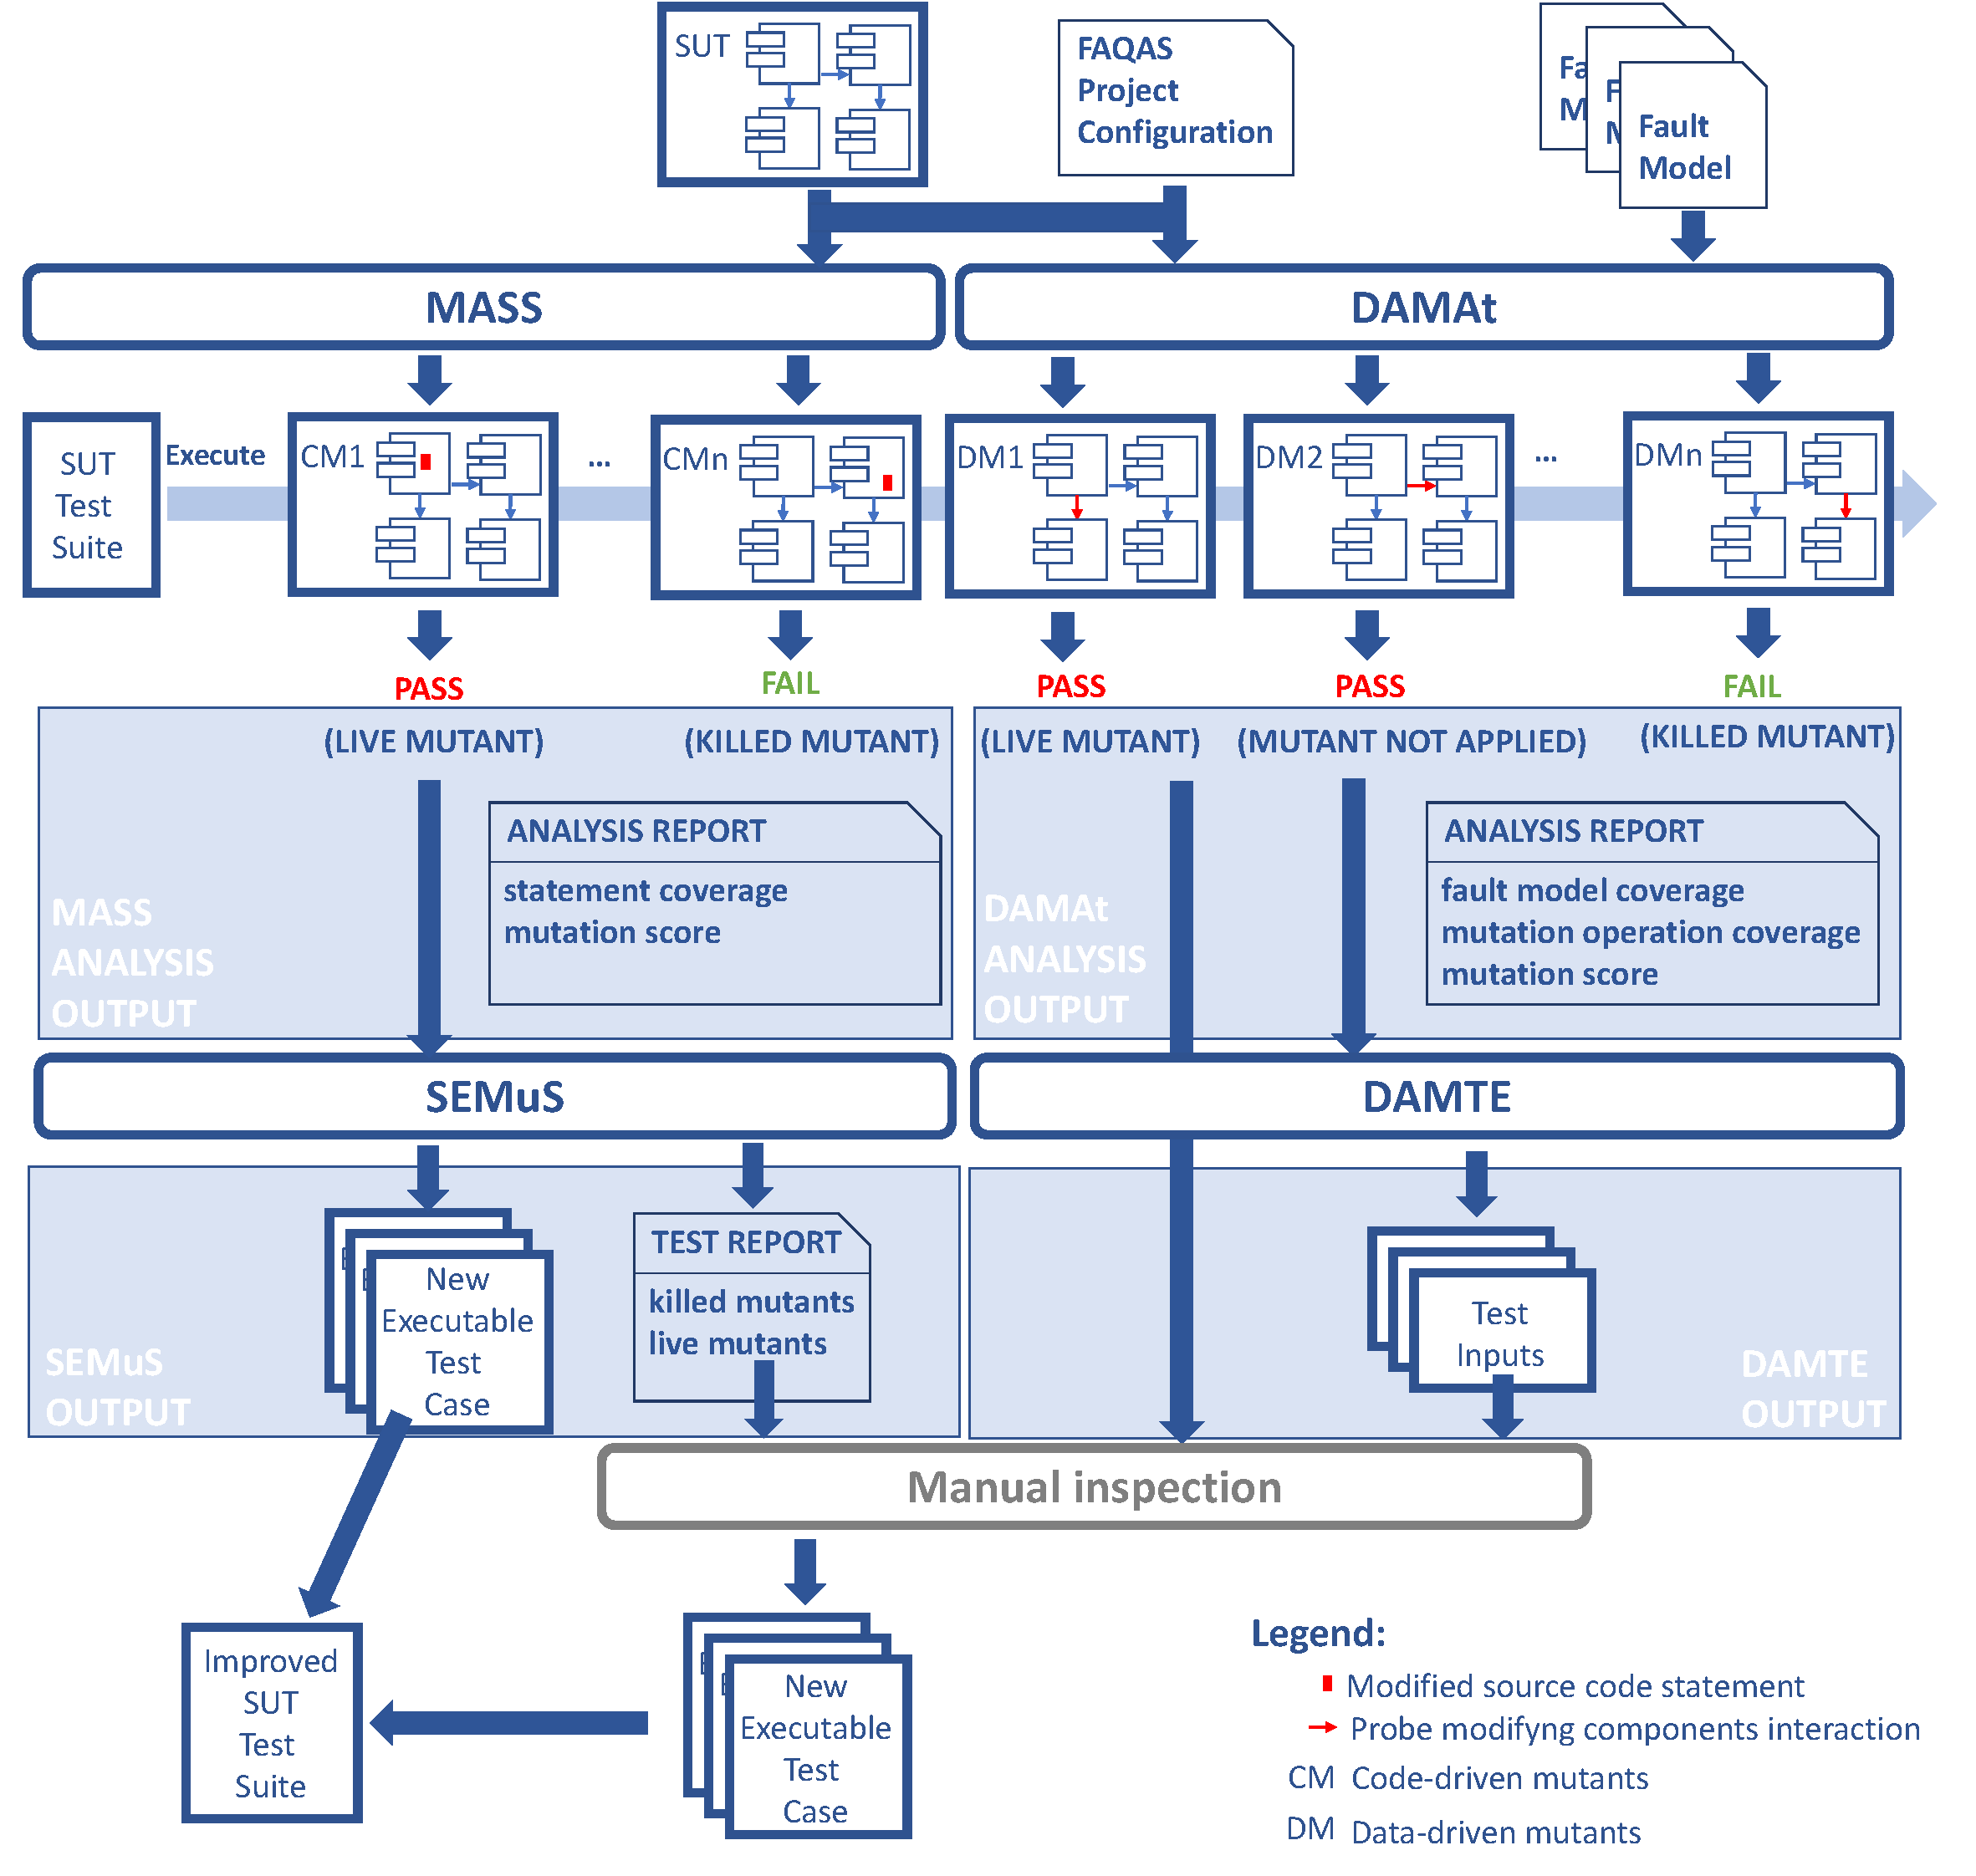
\includegraphics[width=\textwidth]{images/FAQAS-overview.pdf}
\caption{Overview of the FAQAS toolset}
\label{fig:FAQAS:toolset}
\end{center}
\end{figure*}

Figure~\ref{fig:FAQAS:toolset} provides an overview of the input and outputs of the FAQAS toolset. It relies on the idea of generating multiple modified versions of the software system under test (SUT), some are derived by modifying the implementation of the software (code-driven mutants) other by integrating a mutation API that alters the messages exchanged by the software components of the SUT (data-driven mutants). 
The SUT test suite shall be executed with all the mutants, if it is effective then it shall fail with each of them. The mutants for which a failure is not observed are said to be \EMPH{live} and indicate a pitfall in the test suite.
All the FAQAS tools take as input the software under test (SUT), its test suite, and a set of configuration files. 

\EMPH{MASS} generates code-driven mutants. It integrates a pipeline of solutions that make mutation analysis feasible wit large SUT. The three main contributions of MASS are (1) the automated identification of trivially equivalent mutants using an ensemble of compiler optimization options, (2) the computation of the mutation score based on mutant sampling with fixed size confidence interval approach (FSCI), (3) the automated identification of equivalent mutants based on coverage. 
MASS reports the set of live mutants, the set of killed mutants (i.e., mutants that are discovered by the test suite), and information useful to draft a verification report, which includes the statement coverage of the SUT test suite and the mutation score (i.e., the percentage of mutants discovered by the test suite).

\EMPH{DAMAt} generates mutants for data-driven mutation analysis. Data-driven mutation analysis is a research contribution of FAQAS. Instead of mutating the implementation of the SUT, it consists of altering the data exchanged by software components. 
DAMAt relies on fault models that specify how to mutate the data exchanged by software components through data-driven mutation operators. DAMAt can automatically alter data that is stored in data buffers (e.g., before serialization on the communication channel).
DAMAt enables the simulation of faults that affect simulated components (e.g., sensors), which is not feasible with traditional, code-driven mutation analysis. 
DAMAt generates as output a set of killed mutants (i.e., mutants that, during testing, successfully alter the data, and lead to test case failures), a set of live mutants (i.e., mutants that, during testing, successfully alter the data, but do not lead to test case failures), and a set of mutants not applied (i.e., mutants that, during testing, could not alter any data because the data they target is never exercised by the SUT); also, it provides information useful to draft a verification report, which includes the fault model coverage (i.e., percentage of fault models with at least one mutant applied), the mutation operation coverage (i.e., percentage of mutants applied), and the mutation score.

\EMPH{SEMuS} automatically generates executable unit test cases based on code-driven mutation analysis results. The generated unit test cases detect mutants not detected by the original test suite. The generated test cases include test oracles that shall be manually validated by engineers, which enables detecting faults. The generated test cases can be integrated into regression test suites.

SEMuS takes as input the list of live mutants detected by MASS. It generates a set of additional test cases that can be integrated into the SUT test suite. Also, it reports the list of killed mutants and the list of mutants that remain live (i.e., for which SEMuS did not generate a test case that kill them). Live mutants shall be manually inspected by engineers to either determine if they are equivalent or to manually derive a test case capable of killing them.

\EMPH{DAMTE} is a manual procedure supported by an automated symbolic execution toolset; it automatically identifies the test inputs that make software components exchange the data targeted by data-driven mutation operators. The derived test inputs can then be manually integrated into the SUT test suite.
 
%The activity also included an extensive empirical evaluation demonstrating the feasibility, effectiveness, and scalability of the proposed toolsets in the space context, as described in the following sections.

\STARTCHANGEDWPT

\subsection{Objectives}

The FAQAS activity had the following two main objectives:
\begin{itemize}
\item[O1] Searching for an alternative or complementary method of measuring the effectiveness of a test suite (i.e. test-suite verification).
\item[O2] Searching for an alternative or complementary method to build a test suite (i.e. test cases generation).
\end{itemize}

Concerning \emph{O1}, FAQAS led to the development of tools (i.e., MASS and DAMAt) that enable the assessment of test suites by simulating different types of faults (implementation errors and high-level integration problems). Empirical evaluation with software provided by project partners and ESA has shown that the toolset enables detecting relevant test suite limitations (i.e., lack of assertions to verify results, relevant inputs not being tested). Also, it showed that the inspection of mutants enable detecting bugs that affect the software. Finally, preliminary projections made by consortium partners show that the cost of test suite assessment using the FAQAS tools (i.e., engineers' effort) are justified by the highly-valuable benefits (e.g., detection of test suite and software limitations during early development stages, potential avoidance of failures in deployed software).

Concerning \emph{O2}, FAQAS has shown that tools based on symbolic execution (i.e., SEMuS and DaMTE) can automatically generate test cases that detect mutants not detected by the test suite under analysis. However, the research performed in FAQAS has shown that 
symbolic execution tools
are affected by a number of limitations (e.g., dealing with floating point instructions and external components) that limit the feasibility of fully automated test generation. Indeed, only unit test cases not involving complex floating point operations can be automatically generated with state-of-the-art solutions including the FAQAS toolset.

Below, we report on how FAQAS contributed to address the \textbf{detailed objectives} of the activity:
\begin{itemize}
\item {\emph{\textbf{Detailed Objective 1}: To perform a comprehensive analysis and survey of mutation testing.}}

%
%- 
%- 
%- 
%- To define and develop the corresponding toolset supporting this methodology.
%- 

FAQAS has delivered a comprehensive survey of the software engineering literature on mutation testing with the following main findings:
\begin{itemize}
\item	The literature on mutation analysis/testing mostly focuses on modifying the code of the software under test (hereafter, code-driven approaches). Some approaches rely on modifying models, but they aim to generate test cases not assessing test suites. There are no approaches that assess test suites by changing the data generated by software components (hereafter, data-driven approaches).
\item The mutation operators widely adopted to perform code-driven mutation analysis are the sufficient set of operators and the set of deletion operators. Other operators did not receive the same degree of attention in the literature. For example, higher-order mutation operators are reported to be easier to kill than the first-order ones (i.e., they are less effective in assessing test suites limitations); consequently, they had been adopted less in empirical studies.                   
\item The literature lacks mutation analysis approaches that enable simulating errors in the presence of simulated components (e.g., sensors). 
\item Scalable approaches targeting mutation testing (i.e., automatically generating test cases that kill mutants) are few. The most promising ones rely on symbolic execution based on LLVM, which might be inapplicable for onboard flight software compiled for specific architectures. 
\end{itemize}

\item {\emph{\textbf{Detailed Objective 2}: To prototype the mutation testing process to be applied on space software.}}
FAQAS has conducted a detailed analysis and preliminary experiments to select the existing mutation analysis, fault injection, fuzzing, and test generation tools that demonstrated to be reusable for the definition of an automated mutation testing toolset. Some results of the FAQAS evaluation are reported in the following. 
\begin{itemize}
\item	Most existing mutation analysis tools rely on the mutation of LLVM~\cite{LLVM} bitcode, which is often infeasible with space software projects. 
\item The most advanced data mutation tool is the Peach fuzzer~\cite{PeachMozilla}; however, since it has been developed for other purposes (e.g., fuzzing web applications or desktop utilities) it presents an architecture that can hardly be adapted to mutate data in real-time space software. 
\item The automated selection of test inputs that can kill mutants might be supported by either bounded model checking (BMC)~\cite{CBMC} or symbolic execution~\cite{cadar2008klee}; however, existing symbolic execution tools (e.g., KLEE-SEMu~\cite{SEMU}) are more stable and professional than BMC ones. 
\item Finally, complex test inputs (e.g., sequences of hierarchical structures) might be generated by model-based approaches; however, advanced academic tools remain in a prototype state. 
\item The analysis led to the identification of SRCIror~\cite{hariri2018srciror} and KLEE/SEMu as tools that might be extended to build the code-driven components of the FAQAS toolset. Data-driven approaches, instead, need to be built from scratch.
\end{itemize}

\item {\emph{\textbf{Detailed Objective 6}: To define and develop the mutation testing toolset supporting this methodology.}} The FAQAS project has led to a toolset that includes \textbf{\emph{MASS}} (Mutation Analysis for Space Software, TRL 5), 
\textbf{\emph{DAMAt}} (DAta-driven Mutation Analysis with Tables, TRL 4), 
\textbf{\emph{SEMuS}} (Symbolic Execu\-tion-based MUtant analysis for Space software, TRL 3),
and \textbf{\emph{DAMTE}} (DAta-driven Mutation TEsting, TRL 2). 
Details are provided in Section~\ref{sec:methodology}.


\item {\emph{\textbf{Detailed Objective 3}: To empirically evaluate mutation testing by applying it to space software use cases.}} ESA, LXS, and GSL have provided case study subjects that include utility and networking libraries, support tools, and whole systems. They come with test suites of different nature (unit, integration, and system-level). The heterogeneity of case studies and test suites enabled the evaluation of the mutation analysis and testing approaches in a range of representative scenarios. Details are provided in Section~\ref{chapter:caseStudies}.

\item {\emph{\textbf{Detailed Objective 4}: To evaluate the applicability, scalability, efficiency and effectiveness of the approach in the space domain; and to identify limitations of the approach.}} The project conducted an extensive evaluation of MASS, DAMAT, and SEMuS; also, it conducted a preliminary feasibility study for DAMTE. Our results (details in Section~\ref{sec:summary:results}) show that
\begin{itemize}
\item	MASS enables code-driven mutation analysis in the space context. The most effective solutions to improve scalability and mutation score accuracy are mutants sampling and equivalence metrics based on compiler optimizations, respectively. To guarantee a scalable mutation testing process and the accurate computation of the mutation score, mutants sampling should be based on sequential analysis relying on fixed-width sequential confidence interval, a research discovery done within FAQAS.
\item	DAMAt enables an efficient detection of relevant test suite shortcomings with less mutants to be inspected than MASS. It enabled the detection of a range of limitations including message types not being exchanged between software components,  input partitions not being tested, imprecise oracles.
\item SEMuS shows that symbolic execution can be successfully used to select test inputs that kill live mutants within unit test cases. However, unsurprisingly, it cannot be adopted when it is necessary to rely on external components (e.g., networks or simulators), in such cases, which are common for integration and system test suites, symbolic execution alone is insufficient to generate test cases.
\item DAMTE is largely affected by the problems affecting SEMuS with the consequence that it requires large manual effort to be used.
\end{itemize}

\item {\emph{\textbf{Detailed Objective 5}: To evaluate how mutation testing can be integrated into a typical verification \& validation life cycle of space software, and to define the mutation testing methodology.}} FAQAS has provided preliminary ideas about the definition of guidelines for the adoption of mutation analysis and testing strategies within ECSS activities (see Section~\ref{sec:isvv}). The proposed guidelines support both quality assurance activities described in ECSS standards~\cite{ecss40C,ecss80C} and Independent Software Verification and Validation (ISVV) practices~\cite{ESAISVV}. Finally, FAQAS has delivered a method for the assessment and improvement of software based on the results produced by the FAQAS toolset.

\item {\emph{\textbf{Detailed Objective 7}: To foster the use of this methodology among the different software and independent software verification and validation suppliers.}} The FAQAS toolset has been delivered to the project industry partners (i.e., GomSpace and LuxSpace), who validated it  (see Section \ref{sec:validationsum}). Also, the description and empirical results concerning some of the tools part of the FAQAS toolset have been described in papers submitted to top academic venues in the field of software engineering. A paper concerning MASS has already been published in IEEE Transactions on Software Engineering~\cite{Oscar:MASS:TSE}. Adoption among practitioners is a longer term objective that will be targeted during the maintenance phase of the project.

\end{itemize}



\subsection{Outputs}

The activity lead to the following tangible outputs:
\begin{itemize}
\item Tool: MASS. It reaches TRL 5: it is a configurable tool, with a user manual, that can be applied to whole software systems to perform mutation analysis. It has been installed on third party premises (i.e., GSL and LXS development environment)  and independently used by third-party engineers (i.e., GSL and LXS) on relevant cases (e.g., projects not shared with SnT).
\item Tool: DAMAt. It reaches TRL 4: it is a configurable tool, with a user manual, that can be applied to whole software systems to perform mutation analysis. It has been installed on third party premises (i.e., GSL and LXS development environment)  and independently used by third-party engineers (i.e., GSL and LXS) on the case study subjects of the project.
\item Tool: SEMuS. It reaches TRL 3: it is a configurable tool, with a user manual, that can be applied to a subset of source files for space software systems to perform test generation. It has been installed on third party premises (i.e., GSL and LXS development environment)  and independently used by third-party engineers (i.e., GSL and LXS) on a subset of source files belonging to the case study subjects of the project. 
\item Tool: DAMTE. It reaches TRL 2: it is provided as an extension of DAMAt, manual effort and scaffolding is needed to apply it to new projects. It has been applied to one case study subject of the project.
\item E40C/Q80C documentation for the FAQAS toolset; it includes SVS, SValR, SUTR, SUTP, SUM, SSS, SRF, SRelD, SPAP, SDD, SCF, IRD.
\item Demonstration videos for MASS, DAMAt, and SEMuS.
\item Research paper about MASS methodology published in IEEE Transactions on Software Engineering\cite{Oscar:MASS:TSE}.
\item Research paper about DAMAt submitted to ICSE'22.
\item Research paper about MASS tool submitted to ICSE'22.
\end{itemize}

\ENDCHANGEDWPT


%•	An extensive empirical evaluation demonstrating the feasibility of code-driven mutation analysis in the space context. The evaluation has shown that the most effective solutions to improve scalability and mutation score accuracy are mutants sampling and equivalence metrics based on compiler optimizations, respectively. To guarantee a scalable mutation testing process and the accurate computation of the mutation score, mutants sampling should be based on sequential analysis relying on fixed-width sequential confidence interval, a research discovery done within FAQAS.
%•	The definition of an approach, called data-driven mutation analysis, that, instead of mutating the implementation of the software under test, alters the data exchanged by software components. Data-driven mutation analysis enables the injection of faults that affect simulated components (e.g., sensors), which is not feasible with traditional, code-driven mutation analysis.
%•	An empirical evaluation demonstrating the feasibility of data-driven mutation analysis with space software.
%•	The definition of an approach for code-driven mutation testing that relies on symbolic execution to identify test inputs that enable killing mutants not killed by the test suite under analysis.
%•	Demonstrating the feasibility of automated test generation for mutation testing based on symbolic execution. More precisely, symbolic execution can be successfully used to select test inputs that kill live mutants within unit test cases. However, unsurprisingly, it cannot be adopted when, to kill a mutant, it is necessary to rely on external components (e.g., networks or simulators), in such cases, which are common for integration and system test suites, symbolic execution alone is insufficient to generate test cases (e.g., because it cannot translate the simulator logic into an SMT formula to derive test cases from).
%•	The definition of guidelines for the adoption of mutation analysis and testing strategies within ECSS activities. The proposed guidelines support both quality assurance activities described in ECSS standards [2,3] and Independent Software Verification and Validation (ISVV) practices [8].
%•	The delivery of a toolset that implements code-driven mutation analysis, data-driven mutation analysis, and code-driven mutation testing. The toolset includes the following tools:
%o	MASS (Mutation Analysis for Space Software), a tool that automatically executes all the steps of the code-driven mutation analysis methodology developed by the project.
%o	DAMA (DAta-driven Mutation Analysis), a tool that automatically executes all the steps of the data-driven mutation analysis methodology developed by the project.
%o	SEMuS (Symbolic Execution-based MUtant analysis for Space software), a tool that automatically generates test inputs to augment existing test suites. It relies on state-of-the-art solutions [7].
%

%FAQAS.drawio.pdf

%Sections~\ref{ch:mass:approach} to~\ref{sec:data:test_suite_augmentation} provide an overview of the FAQAS tools: MASS, SEMuS, DAMAt, and DAMTE.
%Section~\ref{chapter:caseStudies} introduces the case study subjects considered for empirical evaluation.
%Section~\ref{sec:summary:results} provides an overview of the empirical results obtained.
%Section~\ref{sec:conclusion} concludes this report.

